\subsection{Markov Chains}

This subsection presents a guide on how to use the \texttt{ambulance\_game}
library to create and solve the Markov chain (MC) model of the hospital network
discussed in this thesis (see Chapter~\ref{sec:queueing_section}).
The parameters used are defined in Listing~\ref{lst:abg_how_to_markov}.
For more information on the parameters, refer to
Section~\ref{sec:queueing_section}.


\begin{lstlisting}[
    style=pystyle,
    caption={Python code for the parameters used in the Markov chain model.},
    label={lst:abg_how_to_markov},
]
>>> lambda_1 = 1
>>> lambda_2 = 2
>>> mu = 5
>>>
>>> num_of_servers = 1
>>> threshold = 2
>>> system_capacity = 3
>>> buffer_capacity = 1

\end{lstlisting}

This section focuses on the \texttt{markov} module of the ambulance\_game
library which focuses on the Markov model.
Function \texttt{build\_states} takes in the \texttt{threshold}, the
\texttt{system\_capacity} and the \texttt{buffer\_capacity} variables and
returns a list of all the states of the MC model.

\begin{lstlisting}[
    style=pystyle,
    caption={Python code for building the states of the Markov chain model.},
    label={lst:abg_how_to_markov_states},
]
>>> import ambulance_game as abg
>>> all_states = abg.markov.build_states(
...     threshold=threshold,
...     system_capacity=system_capacity,
...     buffer_capacity=buffer_capacity,
... )
>>> all_states
[(0, 0), (0, 1), (0, 2), (1, 2), (0, 3), (1, 3)]

\end{lstlisting}

To visualise the list of states that are returned by the
\texttt{build\_states} function, the \texttt{visualise\_markov\_chain}
function can be used.

\definecolor{invisiblecomments}{RGB}{253, 246, 220}
\begin{lstlisting}[
    style=pystyle,
    caption={Python code for visualising the Markov chain model.},
    label={lst:abg_how_to_markov_visualise},
    commentstyle=\color{invisiblecomments},
]
>>> abg.markov.visualise_markov_chain(
...     num_of_servers=num_of_servers,
...     threshold=threshold,
...     system_capacity=system_capacity,
...     buffer_capacity=buffer_capacity,
... ) # doctest: +SKIP
\end{lstlisting}

\begin{figure}[H]
    \centering
    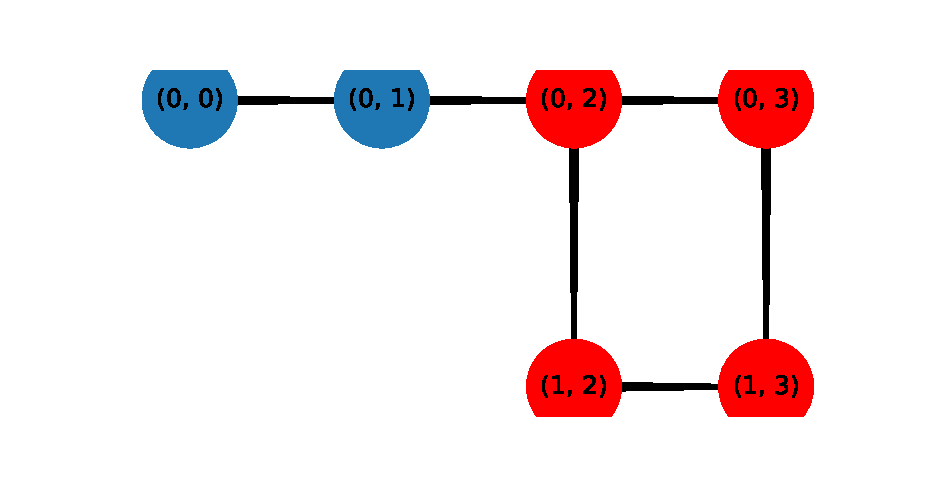
\includegraphics[width=\textwidth]{chapters/00_appendix/01_ambulance_game_library/Bin/visualise_markov.eps}
\end{figure}

The function \texttt{get\_transition\_matrix} builds the transition matrix
of the MC model.

\begin{lstlisting}[
    style=pystyle,
    caption={Python code for building the transition matrix of the Markov
    chain model.},
    label={lst:abg_how_to_markov_transition},
]
>>> Q = abg.markov.get_transition_matrix(
...     lambda_1=lambda_1,
...     lambda_2=lambda_2,
...     mu=mu,
...     num_of_servers=num_of_servers,
...     threshold=threshold,
...     system_capacity=system_capacity,
...     buffer_capacity=buffer_capacity,
... )
>>> Q
array([[-3.,  3.,  0.,  0.,  0.,  0.],
       [ 5., -8.,  3.,  0.,  0.,  0.],
       [ 0.,  5., -8.,  2.,  1.,  0.],
       [ 0.,  0.,  5., -6.,  0.,  1.],
       [ 0.,  0.,  5.,  0., -7.,  2.],
       [ 0.,  0.,  0.,  5.,  0., -5.]])

\end{lstlisting}

The functions shown in Listing~\ref{lst:abg_how_to_markov_steady_state} can be
used to calculate the steady state probabilities of the MC model.
The steady state probabilities can be calculated using a numerical method or
an algebraic method.
For more information on the methods, refer to
Section~\ref{sec:ambulance_game_explanation}.

\begin{lstlisting}[
    style=pystyle,
    caption={Python code for building the steady state probabilities of the
    Markov chain model.},
    label={lst:abg_how_to_markov_steady_state},
]
>>> pi = abg.markov.get_steady_state_numerically(Q)
>>> pi
array([0.44853393, 0.26912036, 0.16147222, 0.07381587, 0.02306746,
       0.02399016])

>>> pi = abg.markov.get_steady_state_algebraically(Q)
>>> pi
array([0.44853393, 0.26912036, 0.16147222, 0.07381587, 0.02306746,
       0.02399016])
    
\end{lstlisting}

The functions shown in Listing~\ref{lst:abg_how_to_markov_expected_number}
can be used to calculate the expected number of patients in the system,
service area and buffer centre.

\begin{lstlisting}[
    style=pystyle,
    caption={Python code for getting the expected number of patients in the
    Markov chain model.},
    label={lst:abg_how_to_markov_expected_number},
]
>>> import numpy as np
>>> np.round(
...     abg.markov.get_mean_number_of_individuals_in_system(
...         pi=pi, states=all_states
...     ), 3
... )
0.979

>>> np.round(
...     abg.markov.get_mean_number_of_individuals_in_service_area(
...         pi=pi, states=all_states
...     ), 3
... )
0.881

>>> np.round(
...     abg.markov.get_mean_number_of_individuals_in_buffer_center(
...         pi=pi, states=all_states
...     ), 3
... )
0.098

\end{lstlisting}

To get the mean waiting time of patients in the system, the code snippet
shown in Listing~\ref{lst:abg_how_to_markov_waiting} can be used.

\begin{lstlisting}[
    style=pystyle,
    caption={Python code for getting the expected waiting time of individuals
    in the Markov chain model.},
    label={lst:abg_how_to_markov_waiting},
]
>>> np.round(
...     abg.markov.get_mean_waiting_time_using_markov_state_probabilities(
...         lambda_1=lambda_1,
...         lambda_2=lambda_2,
...         mu=mu,
...         num_of_servers=num_of_servers,
...         threshold=threshold,
...         system_capacity=system_capacity,
...         buffer_capacity=buffer_capacity,
...     ), 4
... )
0.1195

\end{lstlisting}

Note that an additional argument \texttt{class\_type} can be used to get the
mean waiting time of type 1 or type 2 individuals that takes values \(0\) and
\(1\), respectively.
The default value of \texttt{class\_type} is set to \texttt{None} which
returns the mean waiting time of all individuals.

To get the mean blocking time of type 2 patients in the system (ambulance
patients), the code snippet shown in
Listing~\ref{lst:abg_how_to_markov_blocking} can be used.

\begin{lstlisting}[
    style=pystyle,
    caption={Python code for getting the expected blocking time of type 2
    individuals in the Markov chain model.},
    label={lst:abg_how_to_markov_blocking},
]
>>> np.round(
...     abg.markov.get_mean_blocking_time_using_markov_state_probabilities(
...         lambda_1=lambda_1,
...         lambda_2=lambda_2,
...         mu=mu,
...         num_of_servers=num_of_servers,
...         threshold=threshold,
...         system_capacity=system_capacity,
...         buffer_capacity=buffer_capacity,
...     ), 4
... )
0.0542

\end{lstlisting}

To get the proportion of individuals that are seen within a time target, the
code snippet shown in Listing~\ref{lst:abg_how_to_markov_proportion} can be
used.

\begin{lstlisting}[
    style=pystyle,
    caption={Python code for getting the proportion of individuals within
    target using the Markov chain model.},
    label={lst:abg_how_to_markov_proportion},
]
>>> np.round(
...     abg.markov.proportion_within_target_using_markov_state_probabilities(
...         lambda_1=lambda_1,
...         lambda_2=lambda_2,
...         mu=mu,
...         num_of_servers=num_of_servers,
...         threshold=threshold,
...         system_capacity=system_capacity,
...         buffer_capacity=buffer_capacity,
...         class_type=None,
...         target=0.5,
...     ), 3
... )
0.791

\end{lstlisting}
